\documentclass[12pt, letterpaper]{article}
\usepackage[utf8]{inputenc}
\usepackage{indentfirst}
\usepackage{graphicx}
\usepackage{setspace}
\usepackage[numbers]{natbib}
\usepackage [autostyle, english = american]{csquotes}
\MakeOuterQuote{"}
\usepackage{layout}
\usepackage[title]{appendix}
\usepackage[justification=centering]{caption}
\usepackage{titlesec}
\usepackage[percent]{overpic}
\usepackage{amsmath}
\usepackage{systeme}
\usepackage{blkarray, bigstrut}
\usepackage{tikz}
\usetikzlibrary{tikzmark}
\usepackage[utf8]{inputenc}
\usepackage{relsize}
\usepackage[nameinlink, capitalize, noabbrev]{cleveref}
\usepackage{tabu}
\usepackage[colorlinks=false, hidelinks, breaklinks]{hyperref}
\usepackage{cleveref}

\begin{document}

\setcounter{secnumdepth}{-1}
\titlespacing*{\section}{0pt}{2\baselineskip}{.33333\baselineskip}
\binoppenalty=\maxdimen
\relpenalty=\maxdimen

%Cover page: 5pts
%Course, subject, name, date
\title{MA348 Numerical Analysis, Optimization of Functions}
\author{David Jefts}
\date{March 25\textsuperscript{th}, 2019}
\begin{titlepage}
	\centering
	\maketitle
	\centering
	\hfill
	\vfill
	\thispagestyle{empty}
\end{titlepage}

\setlength{\voffset}{-0.5in}
\setlength{\headsep}{10pt}

%Introduction: 5pts
%Describe the problem and state objectives
\section{\label{sec:intro}Introduction}
	%Write a code to implement the Golden search method to find the maximum of the function f(x)=2 sin(x)-x2/10. Write a short report on how you implemented your code and what were the results, discuss convergence.
	The goal of this lab was to create a program that could find the maximum (or minimum) of a function using the Golden Search bracketing method. The function below was used for the purpose of this lab and to test the program written to find the minimum and maximum: 
	
	\begin{equation*}{f(x)=2 sin(x)-x^2/10}\end{equation*}

%Theory-Analysis: 5pts
%State assumptions and develop equations
\section{\label{sesc:theory}Theory-Analysis}
	 There were no special equations used in this lab, nor were there any assumptions made. The method used was a bracketing method based on the Golden Ratio ($\varphi=0.61803$), as explained in Section \ref{sec:solution}, and the Matrix Row Operations, row switching, row multiplication, and row addition. Row switching is swapping the position of one row with another row. Row multiplication is multiplying a row by a constant. Row addition is replacing a row by the sum of that row and some multiple of another row.

	 
%Numerical Solution: 20pts
%Describe the numerical methods used to solve the problem
\section{\label{solution}Numerical Solution}
	The entirety of the Gaussian Elimination was coded in Python, with the matrices displayed created in \LaTeX{}.
	
	Gaussian Elimination has two major steps, with two optional steps that are discussed at the end of this section. Forward Elimination, which solves the bottom half of the matrix, followed by Backwards Substitution, which solves for the variable values.
	 
	 By the end of the Forward Elimination step, the bottom left-hand corner of the matrix, as highlighted below, should be all equivalent to 0. \vspace{\baselineskip}
	
	This is accomplished through a multi-step algorithm. Below is a walkthrough of the method using the matrix mentioned in the introduction. Matrices can be modified by adding and subtracting rows of the matrix from other rows.\vspace{\baselineskip}
	
	Step 1: The first step begins with the first column and the second row. The goal is to make each spot in the bottom left corner equivalent to 0. For the first step the first row of the matrix is subtracted from each of the other rows a number of times until each spot in that column, below the main diagonal, is equivalent to 0. For the second row, adding the first row just once is sufficient to make a zero ($R_2 + R_1 \rightarrow R_2$, where $R_1$ and $R_2$ refer to rows 1 and 2, respectively), in this case the multiplier for the row is $-1$. To add two rows together, sum the values in each of the matching columns independently. The result is the left matrix. Continuing this process on the third row, achieving a 0 in the first column can be done with: $R_2 - (2\times R_1) \rightarrow R_2$ and the result is the right matrix, in this case the multiplier would be 2.
	
	\begin{center}
		\begin{blockarray}{cccc}
			\begin{block}{ [ ccc !{\color{darkgray}\vrule} c ]}
				\bigstrut[t]
				 1 & -1 &  3 & -3 \\
				 0 &  -1 & 1 &  -2 \\
				 2 &  2 &  4 &  0 \bigstrut[b] \\
			\end{block}
		\end{blockarray}
		\hspace{1cm}
		\begin{blockarray}{cccc}
			\begin{block}{ [ ccc !{\color{darkgray}\vrule} c ]}
				\bigstrut[t]
				 1 & -1 &  3 & -3 \\
				 0 &  -1 & 1 &  -2 \\
				 0 &  4 &  -2 &  6 \bigstrut[b] \\
			\end{block}
		\end{blockarray}
	\end{center}
	
	Step 2: The second step is the same process as the first step, but using the second row to make the second column, below the main diagonal, equivalent to 0. For the third row, achieving a 0 in the second column can be done with: $R_2 + (4\times R_1) \rightarrow R_2$ and the result is the matrix below.
	
	\begin{center}
		\begin{blockarray}{cccc}
			\begin{block}{ [ ccc !{\color{darkgray}\vrule} c ]}
				\bigstrut[t]
				 1 & -1 &  3 & -3 \\
				 0 &  -1 & 1 &  -2 \\
				 0 &  0 &  2 &  -2 \bigstrut[b] \\
			\end{block}
		\end{blockarray}
	\end{center}
	
	The next major step of the Gaussian Elimination Method is Backwards Substitution. Backwards substitution finds the final solution, by converting the matrix back into a system of equations and solving `up' the matrix to find all of the x values.
	
	\begin{center}
		\begin{blockarray}{cccc}
			\begin{block}{ [ ccc !{\color{darkgray}\vrule} c ]}
				\bigstrut[t]
				 1 & -1 &  3 & -3 \\
				 0 &  -1 & 1 &  -2 \\
				 0 &  0 &  2 &  -2 \bigstrut[b] \\
			\end{block}
		\end{blockarray}
		\scalebox{1.75}{$\rightarrow$}
		\systeme{x-y+3z=-3, -y+z=-2, 2z=-2}
	\end{center}
	
	$z$ can now easily be solved for, resulting in $-1$. Substitute $z$ into the second equation to find $y$, then substitute $y$ and $z$ into the first equation to calculate $x$. Then the matrix is solved.
	\vspace{\baselineskip}
	
	Two minor methods that are not always necessary for the Gaussian Elimination Method are Scaling and Partial Pivoting. Scaling is dividing each element by the highest value in a given row. This scales down the matrix so that no number is greater than 1. This can reduce the complexity of the matrix and help it be more readable, but it also increases the chance of round-off errors in computers since some fractions cannot be well-represented digitally. 
	
	Partial Pivoting is required if, at any point in the Forward Elimination Step, a number in the main diagonal is equivalent to 0. This causes errors when finding the multiplier since numbers cannot be divided by 0. Partial Pivoting is the swapping of two rows so that the number on the main diagonal is not 0. The current row is swapped with the row that has the highest absolute value for the column currently being worked on. So if the current row has a 0 in the 3rd column and this 0 is on the main diagonal, then the Partial Pivot would swap the current row with whichever row has the greatest absolute value in the 3rd column.


%Results and Discussion: 45pts
%Tabulate and plot the results, compare results, and discuss the accuracy of results
\section{\label{sec:results}Results and Discussion}
    	The table of the $a$ and $b$ values as described in Section \ref{sec:solution} is shown below:\vspace{\baselineskip}
	
	\begin{center}
	\begin{tabular}{|c|c|c|}
		\hline
		hello & hello & hello \\
		\hline
	\end{tabular}
	\end{center}


%Conclusions: 20pts
%Comment on the efficiency of the solvers
\section{\label{conclusion}Conclusions}
	The Gaussian Elimination Method is very effective at solving matrices, however it has a high operation cost, at $O(n)=O(\frac{2}{3}n^3) + O(n^2)$. Additionally, the method may require the entire matrix to be scaled beforehand which can increase the chance of rounding error when solving with a computer, and certain matrices require pivoting which slightly increases the overall complexity. In conclusion, the Gaussian Elimination Method is very effective at solving matrices and guarantees a solution, but it sacrifices operational power to do so. 

\pagebreak


%Appendices
%Include listings of the source codes, include printed copies of the output files
\appendix
	\section{Appendix A}
            		\begin{figure}[htp]
            			\centering
            			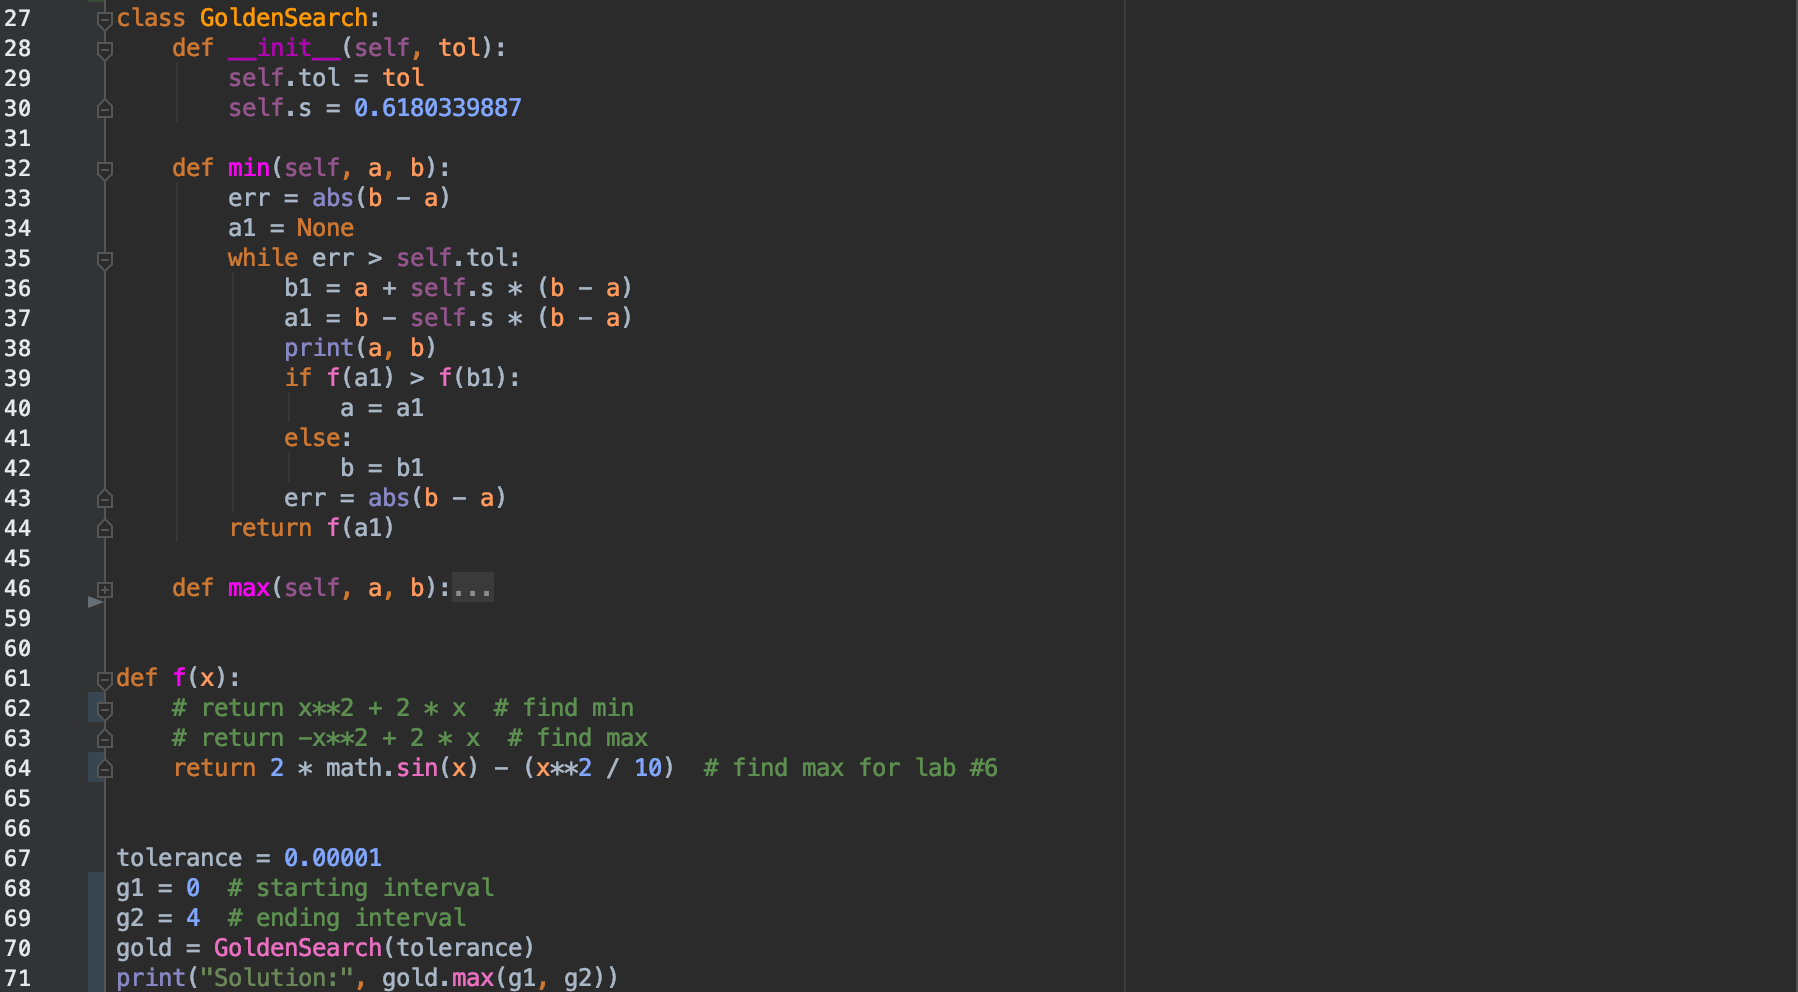
\includegraphics[width=1.0\linewidth]{PythonCode.png}
            		\end{figure}


\end{document}
